\documentclass[11pt,a4paper]{article}

% Packages
\usepackage[utf8]{inputenc}
\usepackage[T1]{fontenc}
\usepackage{mathpazo}
\usepackage{geometry}
\geometry{a4paper, margin=1in}
\usepackage{graphicx}
\usepackage{float}
\usepackage{array}
\usepackage{booktabs}
\usepackage{caption}
\usepackage{xcolor}
\usepackage{tikz}
\usepackage{fancyhdr}
\usepackage{titlesec}
\usepackage{hyperref}
\usepackage{enumitem}
\usepackage{tcolorbox}
\usepackage{colortbl}

% Colors
\definecolor{primary}{HTML}{2C3E50}
\definecolor{accent}{HTML}{8E44AD}
\definecolor{retentiongreen}{HTML}{27AE60}
\definecolor{churnred}{HTML}{E74C3C}
\definecolor{warningorange}{HTML}{F39C12}
\definecolor{lightgray}{HTML}{ECF0F1}

% Hyperlinks
\hypersetup{
    colorlinks=true,
    linkcolor=accent,
    urlcolor=accent,
    citecolor=accent
}

% Headers
\pagestyle{fancy}
\fancyhf{}
\fancyhead[L]{\color{primary}\small Customer Retention \& Churn Analysis}
\fancyhead[R]{\color{primary}\small Future Interns - DS Task 2}
\fancyfoot[C]{\thepage}
\renewcommand{\headrulewidth}{0.4pt}

% Section formatting
\titleformat{\section}
  {\color{primary}\Large\bfseries}
  {\thesection}{1em}{}[\titlerule]
\titleformat{\subsection}
  {\color{accent}\large\bfseries}
  {\thesubsection}{1em}{}

\begin{document}

% =============================================
% COVER PAGE
% =============================================
\begin{titlepage}
    \begin{tikzpicture}[remember picture, overlay]
        \fill[accent] (current page.north west) rectangle (current page.north east);
        \fill[primary] (current page.north west) rectangle ([yshift=-8pt]current page.north east);
        \fill[accent, opacity=0.3] (current page.north west) rectangle ([xshift=4pt]current page.south west);
        \fill[primary] (current page.south west) rectangle ([yshift=4pt]current page.south east);
    \end{tikzpicture}
    
    \vspace*{3cm}
    
    \begin{center}
        {\color{primary}\fontsize{26}{32}\selectfont\bfseries Customer Retention}\\[8pt]
        {\color{primary}\fontsize{26}{32}\selectfont\bfseries\& Churn Analysis}
        
        \vspace{1.5cm}
        
        {\color{accent}\Large Statistical Analysis with Business Recommendations}
        
        \vspace{2cm}
        
        \begin{tcolorbox}[
            colback=lightgray,
            colframe=accent,
            boxrule=0.5pt,
            arc=4pt,
            width=0.8\textwidth,
            center
        ]
            \begin{center}
                {\color{primary}\large\textbf{Future Interns}}\\[4pt]
                {\color{primary}Data Science \& Analytics - Task 2}\\[4pt]
                {\color{primary}Customer Retention \& Churn Analysis}
            \end{center}
        \end{tcolorbox}
        
        \vspace{2.5cm}
        
        {\color{primary}\large\textbf{Prepared by:} Thembinkosi Phama}\\[6pt]
        {\color{primary}\large\textbf{Date:} \today}\\[6pt]
        {\color{primary}\large\textbf{Repository:} FUTURE\_DS\_02}
        
        \vfill
        
        \begin{center}
            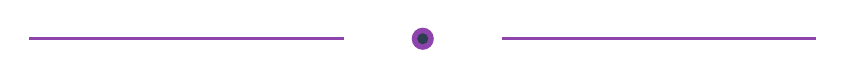
\begin{tikzpicture}
                \draw[accent, line width=1pt] (0,0) -- (4,0);
                \draw[accent, line width=1pt] (6,0) -- (10,0);
                \fill[accent] (5,0) circle (4pt);
                \fill[primary] (5,0) circle (2pt);
            \end{tikzpicture}
        \end{center}
    \end{center}
\end{titlepage}

% =============================================
% TABLE OF CONTENTS
% =============================================
\newpage
\renewcommand{\contentsname}{\color{primary}\Large\bfseries Table of Contents}
\tableofcontents
\newpage

% =============================================
% EXECUTIVE SUMMARY
% =============================================
\section{Executive Summary}

\begin{tcolorbox}[
    colback=accent!5,
    colframe=accent!40,
    arc=8pt,
    left=15pt,
    right=15pt,
    top=12pt,
    bottom=12pt
]
This report analyzes \textbf{7,043 customers} from a telecommunications company to identify churn patterns, key risk factors, and retention strategies. Using chi-square tests and logistic regression, we identify the strongest predictors of customer churn and provide evidence-based recommendations.
\end{tcolorbox}

\vspace{12pt}

\subsection{Key Performance Indicators}

\begin{table}[H]
\centering
\begin{tabular}{p{5cm} p{5cm}}
\toprule
\rowcolor{primary!10}
\textbf{Metric} & \textbf{Value} \\
\midrule
Total Customers & 7,043 \\
\textbf{Churn Rate} & \textbf{26.54\%} \\
Churned Customers & 1,869 \\
Retained Customers & 5,174 \\
Avg Monthly Charge & \$64.76 \\
\textbf{Monthly Revenue at Risk} & \textbf{\$121,040} \\
\textbf{Yearly Revenue at Risk} & \textbf{\$1,452,475} \\
\bottomrule
\end{tabular}
\caption{Churn Key Performance Indicators}
\end{table}

\begin{tcolorbox}[
    colback=churnred!5,
    colframe=churnred!40,
    arc=8pt,
    left=12pt,
    right=12pt
]
\textbf{Critical Finding:} Over 1 in 4 customers churn, putting \textbf{\$1.45 million} in annual revenue at risk. Month-to-month contracts (42.7\% churn), Fiber Optic service (41.9\%), and Electronic Check payments (45.3\%) are the strongest risk factors identified.
\end{tcolorbox}

% =============================================
% DATA OVERVIEW
% =============================================
\section{Data Overview}

\begin{table}[H]
\centering
\begin{tabular}{p{4cm} p{6cm}}
\toprule
\rowcolor{primary!10}
\textbf{Attribute} & \textbf{Description} \\
\midrule
Dataset Source & Telco Customer Churn Dataset \\
Total Customers & 7,043 \\
Features & 21 (demographics, services, billing) \\
Target Variable & Churn (Yes/No) \\
Data Quality & 11 missing TotalCharges (fixed) \\
Duplicate Records & 0 \\
\bottomrule
\end{tabular}
\caption{Dataset Characteristics}
\end{table}

\subsection{Business Questions Addressed}
\begin{enumerate}[label=\color{accent}\textbf{Q\arabic*:}, leftmargin=*]
    \item Why are customers leaving?
    \item Which segments are most at risk?
    \item How long do customers typically stay?
    \item What services correlate with retention?
    \item What actions can reduce churn?
\end{enumerate}

% =============================================
% CHURN ANALYSIS
% =============================================
\section{Churn Analysis Results}

\subsection{Churn by Contract Type}

\begin{table}[H]
\centering
\begin{tabular}{p{4cm} p{2.5cm} p{2.5cm} p{2.5cm}}
\toprule
\rowcolor{primary!10}
\textbf{Contract Type} & \textbf{Customers} & \textbf{Churned} & \textbf{Churn Rate} \\
\midrule
\rowcolor{churnred!15}
Month-to-Month & 3,875 & 1,655 & \textcolor{churnred}{\textbf{42.71\%}} \\
One Year & 1,473 & 166 & 11.27\% \\
\rowcolor{retentiongreen!15}
Two Year & 1,695 & 48 & \textcolor{retentiongreen}{\textbf{2.83\%}} \\
\bottomrule
\end{tabular}
\caption{Churn Rate by Contract Type}
\end{table}

\begin{tcolorbox}[
    colback=churnred!5,
    colframe=churnred!60,
    title=\textbf{Key Finding: Contract Type is the \#1 Predictor},
    fonttitle=\bfseries,
    arc=6pt
]
Month-to-month customers are \textbf{15 times more likely to churn} than two-year contract customers (42.71\% vs 2.83\%). Converting month-to-month customers to annual contracts represents the single biggest retention opportunity.
\end{tcolorbox}

\subsection{Churn by Customer Tenure}

\begin{table}[H]
\centering
\begin{tabular}{p{4cm} p{2.5cm} p{2.5cm} p{2.5cm}}
\toprule
\rowcolor{primary!10}
\textbf{Tenure Group} & \textbf{Customers} & \textbf{Churned} & \textbf{Churn Rate} \\
\midrule
\rowcolor{churnred!15}
0--12 months & 2,186 & 1,037 & \textcolor{churnred}{\textbf{47.44\%}} \\
13--24 months & 1,024 & 294 & 28.71\% \\
25--36 months & 832 & 180 & 21.63\% \\
37--48 months & 762 & 145 & 19.03\% \\
49--60 months & 832 & 120 & 14.42\% \\
\rowcolor{retentiongreen!15}
60+ months & 1,407 & 93 & \textcolor{retentiongreen}{\textbf{6.61\%}} \\
\bottomrule
\end{tabular}
\caption{Churn Rate by Customer Tenure}
\end{table}

\subsection{Churn by Internet Service}

\begin{table}[H]
\centering
\begin{tabular}{p{4cm} p{2.5cm} p{2.5cm} p{2.5cm}}
\toprule
\rowcolor{primary!10}
\textbf{Internet Service} & \textbf{Customers} & \textbf{Churned} & \textbf{Churn Rate} \\
\midrule
\rowcolor{churnred!15}
Fiber Optic & 3,096 & 1,297 & \textcolor{churnred}{\textbf{41.89\%}} \\
DSL & 2,421 & 459 & 18.96\% \\
\rowcolor{retentiongreen!15}
No Internet & 1,526 & 113 & \textcolor{retentiongreen}{\textbf{7.40\%}} \\
\bottomrule
\end{tabular}
\caption{Churn Rate by Internet Service Type}
\end{table}

\subsection{Churn by Payment Method}

\begin{table}[H]
\centering
\begin{tabular}{p{4.5cm} p{2.5cm} p{2.5cm} p{2.5cm}}
\toprule
\rowcolor{primary!10}
\textbf{Payment Method} & \textbf{Customers} & \textbf{Churned} & \textbf{Churn Rate} \\
\midrule
\rowcolor{churnred!15}
Electronic Check & 2,365 & 1,071 & \textcolor{churnred}{\textbf{45.29\%}} \\
Mailed Check & 1,612 & 308 & 19.11\% \\
Bank Transfer (Auto) & 1,544 & 258 & 16.71\% \\
\rowcolor{retentiongreen!15}
Credit Card (Auto) & 1,522 & 232 & \textcolor{retentiongreen}{\textbf{15.24\%}} \\
\bottomrule
\end{tabular}
\caption{Churn Rate by Payment Method}
\end{table}

\subsection{Churn by Senior Citizen Status}

\begin{table}[H]
\centering
\begin{tabular}{p{4cm} p{2.5cm} p{2.5cm} p{2.5cm}}
\toprule
\rowcolor{primary!10}
\textbf{Senior Citizen} & \textbf{Customers} & \textbf{Churned} & \textbf{Churn Rate} \\
\midrule
\rowcolor{retentiongreen!15}
No & 5,901 & 1,393 & \textcolor{retentiongreen}{\textbf{23.61\%}} \\
\rowcolor{churnred!15}
Yes & 1,142 & 476 & \textcolor{churnred}{\textbf{41.68\%}} \\
\bottomrule
\end{tabular}
\caption{Churn Rate by Senior Citizen Status}
\end{table}

% =============================================
% STATISTICAL ANALYSIS
% =============================================
\section{Statistical Analysis}

\subsection{Chi-Square Tests - Identifying Significant Factors}

\begin{tcolorbox}[
    colback=primary!5,
    colframe=primary!50,
    arc=8pt,
    left=12pt,
    right=12pt
]
\textbf{17 out of 19 variables tested} showed a statistically significant relationship with churn (p $<$ 0.05). Only \textbf{Gender} and \textbf{Phone Service} were not significant predictors.
\end{tcolorbox}

\subsection{Cramer's V - Effect Size}

\begin{table}[H]
\centering
\begin{tabular}{p{5cm} p{3cm} p{3cm}}
\toprule
\rowcolor{primary!10}
\textbf{Variable} & \textbf{Cramer's V} & \textbf{Strength} \\
\midrule
Contract Type & 0.410 & Moderate \\
Tenure Group & 0.352 & Moderate \\
Online Security & 0.347 & Moderate \\
Tech Support & 0.343 & Moderate \\
Internet Service & 0.322 & Moderate \\
Payment Method & 0.303 & Moderate \\
Online Backup & 0.292 & Weak \\
Device Protection & 0.282 & Weak \\
Monthly Charges Group & 0.234 & Weak \\
Streaming Movies & 0.231 & Weak \\
Streaming TV & 0.231 & Weak \\
Has Internet & 0.228 & Weak \\
Paperless Billing & 0.192 & Weak \\
Dependents & 0.164 & Weak \\
Senior Citizen & 0.151 & Weak \\
Partner & 0.150 & Weak \\
Multiple Lines & 0.040 & Negligible \\
Phone Service & 0.011 & Negligible \\
Gender & 0.008 & Negligible \\
\bottomrule
\end{tabular}
\caption{Cramer's V Effect Size for All Variables}
\end{table}

\subsection{Logistic Regression - Quantifying Risk}

\textbf{Model:} Churn $\sim$ Contract + Tenure + Internet + Payment + Services + Senior Citizen + Paperless Billing

\begin{table}[H]
\centering
\begin{tabular}{p{4cm} p{3cm}}
\toprule
\rowcolor{primary!10}
\textbf{Metric} & \textbf{Value} \\
\midrule
Pseudo R-squared & 0.2689 \\
Accuracy & 79.81\% \\
Specificity & 90.34\% \\
Sensitivity & 50.67\% \\
AIC & 5,990.85 \\
\bottomrule
\end{tabular}
\caption{Logistic Regression Model Performance}
\end{table}

\subsection{Odds Ratios - What Drives Churn?}

\subsubsection{Factors That INCREASE Churn Risk}

\begin{table}[H]
\centering
\begin{tabular}{p{4.5cm} p{2.5cm} p{4.5cm}}
\toprule
\rowcolor{primary!10}
\textbf{Factor} & \textbf{Odds Ratio} & \textbf{Interpretation} \\
\midrule
\rowcolor{churnred!15}
Fiber Optic Internet & 2.70$\times$ & 170\% higher churn risk \\
Electronic Check Payment & 1.52$\times$ & 52\% higher churn risk \\
Paperless Billing & 1.48$\times$ & 48\% higher churn risk \\
Senior Citizen & 1.37$\times$ & 37\% higher churn risk \\
\bottomrule
\end{tabular}
\caption{Top Churn Risk Increasers}
\end{table}

\subsubsection{Factors That DECREASE Churn Risk}

\begin{table}[H]
\centering
\begin{tabular}{p{4.5cm} p{2.5cm} p{4.5cm}}
\toprule
\rowcolor{primary!10}
\textbf{Factor} & \textbf{Odds Ratio} & \textbf{Interpretation} \\
\midrule
\rowcolor{retentiongreen!15}
Two-Year Contract & 0.17$\times$ & 83\% lower churn risk \\
60+ Months Tenure & 0.19$\times$ & 81\% lower churn risk \\
One-Year Contract & 0.44$\times$ & 56\% lower churn risk \\
No Internet Service & 0.48$\times$ & 52\% lower churn risk \\
\bottomrule
\end{tabular}
\caption{Top Churn Risk Reducers}
\end{table}

\begin{tcolorbox}[
    colback=churnred!5,
    colframe=churnred!60,
    title=\textbf{Statistical Conclusion},
    fonttitle=\bfseries,
    arc=6pt
]
The strongest actionable finding: \textbf{Moving a customer from month-to-month to a two-year contract reduces their churn odds by 83\%}. This single intervention could retain hundreds of customers and save over \$1M in annual revenue.
\end{tcolorbox}

% =============================================
% RECOMMENDATIONS
% =============================================
\section{Recommendations}

\subsection{Immediate Actions (0--3 Months)}

\begin{enumerate}[label=\color{churnred}\textbf{\theenumi.}, leftmargin=*]
    \item \textbf{Launch contract conversion campaign} - Target month-to-month customers with incentives to switch to annual/two-year contracts
    \item \textbf{Address Fiber Optic churn} - Investigate service quality issues; 41.9\% churn suggests product problems
    \item \textbf{Promote automatic payments} - Electronic check users have 45.3\% churn vs 15.2\% for credit card auto-pay
\end{enumerate}

\subsection{Strategic Initiatives (3--12 Months)}

\begin{enumerate}[label=\color{accent}\textbf{\theenumi.}, leftmargin=*]
    \setcounter{enumi}{3}
    \item \textbf{First-year retention program} - 47.4\% churn in first 12 months requires onboarding improvements
    \item \textbf{Senior citizen support} - 41.7\% churn rate; develop specialized retention team
    \item \textbf{Service bundling strategy} - Customers with 7+ services have only 8.7\% churn
\end{enumerate}

\subsection{Estimated Financial Impact}

\begin{tcolorbox}[
    colback=retentiongreen!5,
    colframe=retentiongreen!50,
    arc=8pt,
    left=15pt,
    right=15pt
]
Reducing churn by just \textbf{5 percentage points} (from 26.5\% to 21.5\%) would retain approximately \textbf{350 additional customers} and save \textbf{\$272,000 in annual revenue}.
\end{tcolorbox}

% =============================================
% METHODOLOGY
% =============================================
\section{Methodology}

\begin{table}[H]
\centering
\begin{tabular}{p{4cm} p{7cm}}
\toprule
\rowcolor{primary!10}
\textbf{Technique} & \textbf{Purpose} \\
\midrule
Data Cleaning & Handle missing values, create derived features \\
Descriptive Statistics & Churn rate by segment, KPI calculation \\
Chi-Square Tests & Identify statistically significant churn factors \\
Cramer's V & Measure effect size of each predictor \\
Logistic Regression & Quantify churn risk (odds ratios) \\
Confusion Matrix & Evaluate model performance \\
\bottomrule
\end{tabular}
\caption{Analytical Methodology}
\end{table}

\textbf{Tools Used:} R Statistical Computing Environment, tidyverse, broom, ggplot2

% =============================================
% CONCLUSION
% =============================================
\section{Conclusion}

\begin{tcolorbox}[
    colback=primary!5,
    colframe=primary!50,
    arc=8pt,
    left=15pt,
    right=15pt,
    top=15pt,
    bottom=15pt
]
This analysis identified \textbf{26.54\% churn rate} representing \textbf{\$1.45M in annual revenue at risk}. Statistical testing confirmed that \textbf{17 of 19 variables} significantly predict churn.

\vspace{8pt}

\textbf{The Churn Profile:} The highest-risk customer is on a \textbf{month-to-month contract}, paying by \textbf{electronic check}, using \textbf{Fiber Optic internet}, and in their \textbf{first year} of service. This customer is \textbf{15$\times$ more likely to churn} than a two-year contract customer.

\vspace{8pt}

\textbf{Key Takeaways:}
\begin{itemize}[leftmargin=*]
    \item \textbf{Contract type} is the single strongest predictor -- two-year contracts reduce churn by 83\%
    \item \textbf{First-year retention} is critical -- 47.4\% of new customers leave within 12 months
    \item \textbf{Payment method matters} -- automatic payments show significantly lower churn
    \item \textbf{Service bundling works} -- 7+ services reduces churn to single digits
    \item \textbf{Fiber Optic needs investigation} -- 2.7$\times$ churn risk suggests product issues
\end{itemize}

\vspace{8pt}

The recommendations in this report provide a clear, evidence-based roadmap for reducing churn and protecting over \$1.4M in annual revenue.

\vspace{8pt}

\begin{center}
\textbf{Reducing churn by 5 points = \$272,000 in saved annual revenue}
\end{center}
\end{tcolorbox}

\vspace{1cm}

\begin{center}

\begin{tikzpicture}
    \fill[accent] (0,0) rectangle (15,0.3);
    \fill[primary] (0,0) rectangle (15,0.1);
\end{tikzpicture}

\vspace{6pt}

{\color{primary}\small Report prepared for \textbf{Future Interns - Data Science \& Analytics Task 2}}\\[4pt]
{\color{primary}\small Analysis conducted using R Statistical Computing Environment}\\[4pt]
{\color{primary}\small \today}
\end{center}

\end{document}